\documentclass[t]{beamer}

%\usepackage{verbatim} % writing code 
%\usepackage{listings}
\usepackage{graphicx}
\usepackage{subfig}

\title{Connectivity Graph of WMATA Rail Network}
\author{J. Paz \\{\small contractdesign at gmail.com}}
\date{\today}


\begin{document}

\begin{frame}
\titlepage
\end{frame}

\begin{frame}
\frametitle{Summary}

\begin{block}{Goal}
\begin{itemize}
\item Map the connectivity between the track circuits in the WMATA
  rail network into a human understandable form.
\end{itemize}
\end{block}

\begin{block}{Motivation}
\begin{itemize}
\item Where does a train go after it reaches its destination?
\item Which tracks are being used because of Safetrack?
\item Are there any interesting connections?
\end{itemize}
\end{block}

\end{frame}


%----------------------------------------
\begin{frame}
\frametitle{Logical vs. Physical Views}

\captionsetup[subfigure]{labelformat=empty}
\begin{figure}[!tbp]
  \centering
  \subfloat[Logical View.]{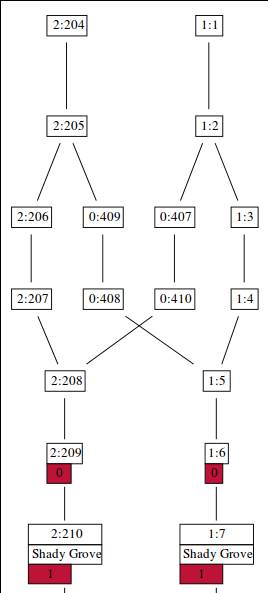
\includegraphics[scale=0.42]{shady_grove_logical.png}}
  \hfill
  \subfloat[Physical View.]{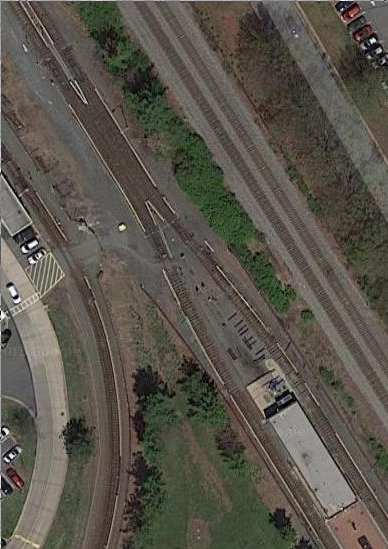
\includegraphics[scale=0.45]{shady_grove_google.png}}
  \footnote{credit:google.com}
\end{figure}


\end{frame}



%----------------------------------------
\begin{frame}
\frametitle{What is a Track Circuit Identifier (CID)?}

A CID is an integer $\{1, 2, .., 3486\}$ returned by the WMATA API indicating the system-wide position of a train.
\begin{itemize}
\item corresponds to a sensor located on the tracks (\href{https://en.wikipedia.org/wiki/Track_circuit}{wiki})
\item location (lat, long) is not available by the API, except for the
  CIDs that correspond to stations.
\end{itemize}

\begin{center}
\begin{figure}
  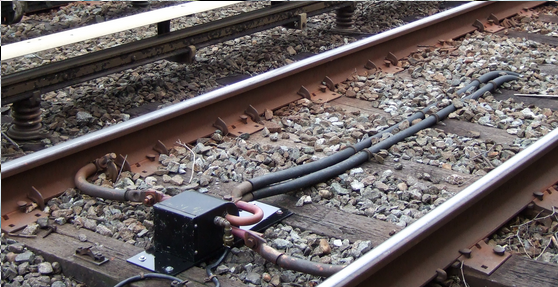
\includegraphics[scale=0.4]{track_sensor.png}
  \footnote{credit: washingtondcmetro.wordpress.com}
\end{figure}
\end{center}
\end{frame}

%----------------------------------------
\begin{frame}
\frametitle{Connectivity Graph}
Each track circuit may be connected to between 1 and 3 other circuits.

\begin{center}
\begin{figure}
  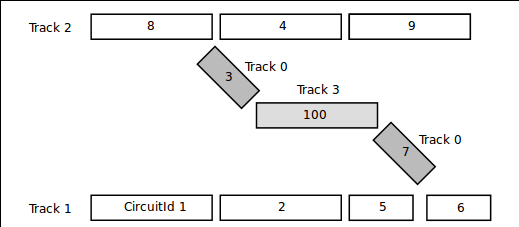
\includegraphics[scale=0.4]{switch.png}
  \footnote{credit:developer.wmata.com}
%  \caption{source: wmata.com)}
\end{figure}
\end{center}

\vfill

The rail network may be viewed as an undirected graph
$G=(V,E)$, where the vertices are the track circuits and the edges are the
connections to the neighboring circuits.

\vfill

With this view we can then leverage graph drawing tools, (e.g., graphviz), to
visualize the network.


\end{frame}


%----------------------------------------
\begin{frame}
\frametitle{Results: Where Does The Train Go?}

Visited CIDs are in magenta.  Train\footnote{Observe how a train skips CIDs when crossing a switch}:
\begin{itemize}
\item switches to/from track 1/2 via 407/409
\item enters/departs system via 1/204
\end{itemize}

\begin{center}
\begin{figure}
  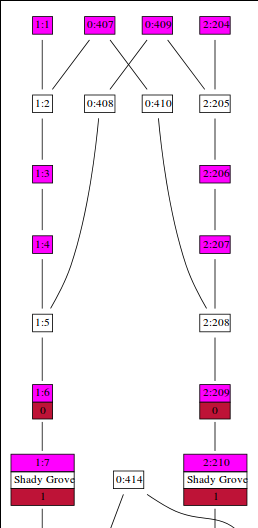
\includegraphics[scale=0.45]{red_line_end.png}
\end{figure}
\end{center}

\end{frame}




%----------------------------------------
\begin{frame}
\frametitle{Results: Safetrack 11/16/2016}

Visited CIDs in magenta.  No traffic seen
between NoMa-Gallaudet and Fort Totten.

\captionsetup[subfigure]{labelformat=empty}
\begin{figure}[!tbp]
  \centering
  \subfloat[NoMa-Gallaudet.]{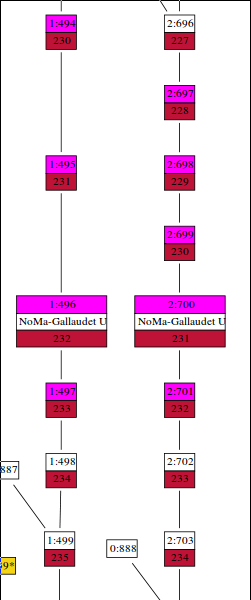
\includegraphics[scale=0.35]{safetrack_noma.png}}
  \hspace{0.75in}
  \subfloat[Ft. Totten.]{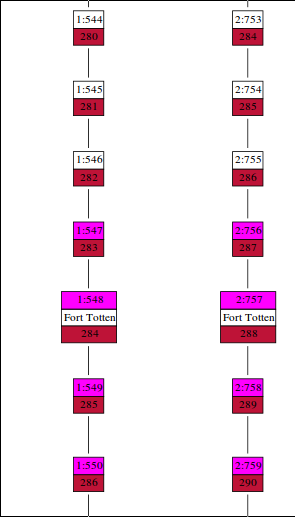
\includegraphics[scale=0.4]{safetrack_totten.png}}

\end{figure}

\end{frame}

%----------------------------------------
\begin{frame}
\frametitle{Results: Surprise Connections}

There is a rail link between between the Red and Blue/Orange/Gray lines.
\begin{center}
\begin{figure}
  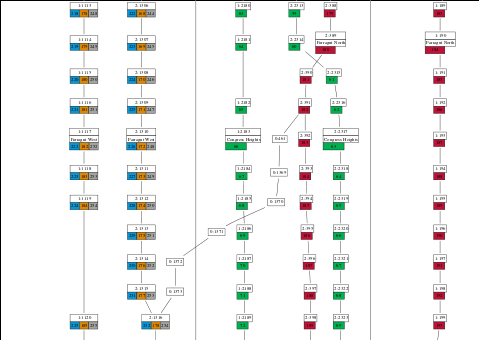
\includegraphics[scale=0.75]{red_to_blue.png}
\end{figure}
\end{center}

\end{frame}

%----------------------------------------
\begin{frame}
\frametitle{Results: Surprise Connections (cont.)}

There is a rail link between between the Red and Green lines.  As a result of these connections, a train can travel to any part of the network (graph is \textit{connected})
\begin{center}
\begin{figure}
  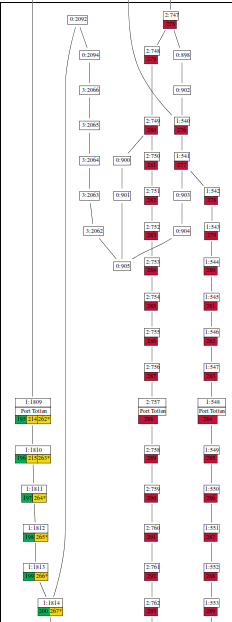
\includegraphics[scale=0.45]{red_to_green.png}
\end{figure}
\end{center}

\end{frame}


%----------------------------------------
\begin{frame}
\frametitle{References}


\begin{block}{Diagrams}
\begin{itemize}
\item \href{https://https://github.com/contractdesign/wmata/blob/master/doc/all.png}{png}
\item \href{https://https://github.com/contractdesign/wmata/blob/master/doc/all.svg}{svg}
\end{itemize}
\end{block}

\begin{block}{Code}
\begin{itemize}
\item \href{https://github.com/contractdesign/wmata/blob/master/doc/make_segments.py}{draw graph}
\item \href{https://github.com/contractdesign/wmata/blob/master/doc/wmata.py}{library}
\end{itemize}
\end{block}


\end{frame}



%----------------------------------------
\begin{frame}
\frametitle{Backup Slides}


\end{frame}


%----------------------------------------
\begin{frame}
\frametitle{Analysis}

\begin{itemize}
\item \href{https://https://github.com/contractdesign/wmata/blob/master/doc/types.txt}{Info on CIDs}
\item \href{https://https://github.com/contractdesign/wmata/blob/master/doc/CircuitIds.txt}{CIDs on each line}
\item \href{https://https://github.com/contractdesign/wmata/blob/master/doc/track_segments.txt}{Continuous sections of track}
\item \href{https://https://github.com/contractdesign/wmata/blob/master/doc/switches.txt}{Switch CIDs}
\item \href{https://https://github.com/contractdesign/wmata/blob/master/doc/ends.txt}{Terminal CIDs}

\end{itemize}


\end{frame}





\end{document}
